% !TeX document-id = {5a531d4e-d456-4a9b-ba5c-fc9e0756255e}
% !TEX TS-program = lualatex
% !BIB TS-program = biber
% Compile: lualatex main && biber main && lualatex main && lualatex main
\begin{filecontents*}{refs.bib}
	@article{Horvath2021DLV,
		title={Deep learning volatility: a deep neural network perspective on pricing and calibration in (rough) volatility models},
		author={Horvath, Blanka and Muguruza, Aitor and Tomas, Mehdi},
		journal={Quantitative Finance},
		volume={21}, number={1}, pages={11--27}, year={2021},
		doi={10.1080/14697688.2020.1817974}
	}
	@misc{Baschetti2024DeepCalibrationRandomGrids,
		title={Deep calibration with random grids},
		author={Baschetti, Fabio and Bormetti, Giacomo and Rossi, Pietro},
		year={2024}, note={arXiv preprint}, url={https://arxiv.org/abs/2306.11061}
	}
	@mastersthesis{Bertolo2024RoughHestonSchemes,
		title={Two simulation schemes for the rough Heston model: a comparison},
		author={Bertolo, Marco}, school={University of Padova}, year={2024}
	}
	@misc{DLVProjectNote,
		title={Deep Learning Volatility: Project Description},
		author={Project Authors},
		year={2025}, note={Internal document}
	}
	
\end{filecontents*}

\documentclass[11pt,a4paper]{report}
\usepackage[english]{babel}
\usepackage{csquotes}
\usepackage[margin=1in]{geometry}
\usepackage{microtype}
% Load math packages BEFORE cleveref
\usepackage{amsmath,amssymb,mathtools}
% Graphics and utilities
\usepackage{graphicx}
\usepackage{subcaption}
\usepackage{booktabs}
\usepackage{siunitx}
\usepackage{tikz}
\usepackage{listings}
\usepackage{xcolor}
\usepackage{enumitem}
% Hyperref BEFORE cleveref
\usepackage{hyperref}
% cleveref AFTER amsmath and hyperref
\usepackage[nameinlink,capitalise]{cleveref}
% biblatex with natbib-compat so \citet/\citep work
\usepackage[backend=biber,style=authoryear,maxbibnames=6,natbib=true]{biblatex}
\addbibresource{refs.bib}

% Listings (Python)
\lstdefinestyle{py}{language=Python, basicstyle=\ttfamily\small, keywordstyle=\color{blue!60!black},
	commentstyle=\color{green!40!black}, stringstyle=\color{red!50!black}, showstringspaces=false,
	frame=single, rulecolor=\color{black!20}, numbers=left, numberstyle=\tiny, numbersep=6pt}

% Stile per codice Python più elegante
\lstdefinestyle{cleanpy}{
	language=Python,
	basicstyle=\ttfamily\footnotesize,
	frame=single,
	rulecolor=\color{black!20},
	backgroundcolor=\color{gray!5},
	showstringspaces=false,
	breaklines=true,
	columns=fullflexible,
	numberstyle=\tiny\color{gray},
	commentstyle=\color{gray!70},
	keywordstyle=\color{black!80}\bfseries,
	stringstyle=\color{black!60},
	aboveskip=6pt,
	belowskip=6pt
}
% Simple TODO macro
\newcommand{\TODO}[1]{\textcolor{red!70!black}{\textbf{TODO:}~#1}}

\title{Deep Learning Volatility\\\large A Modular Framework for Learning and Calibrating Implied Volatility Surfaces}
\author{Bianchi Giacomo}
\date{\today}

\begin{document}
	\maketitle
	\tableofcontents
	
	\chapter{Introduction}
	\label{ch:intro}
	This document describes the \emph{Deep Learning Volatility} (DLV) framework: a modular system to learn, generate, and calibrate implied volatility (IV) surfaces for classical and rough stochastic volatility models. DLV follows a two-step design: (i) an \emph{offline} learning phase where neural networks approximate expensive pricing maps, and (ii) an \emph{online} calibration phase where the surrogate is optimized against market data. Our approach bridges grid-based surface learning \citep{Horvath2021DLV} with pointwise training on \emph{random grids/smiles} \citep{Baschetti2024DeepCalibrationRandomGrids}. We target modern rough models (e.g., rough Heston, rough Bergomi), where direct Monte Carlo or fractional-Riccati methods hinder calibration speed.
	
	\paragraph{Contributions.} This documentation
	\begin{itemize}[nosep]
		\item formalizes the architecture (\cref{ch:overview}),
		\item specifies the stochastic-process interface used by all models (Chapter~\ref{ch:stoch_interface}),
		\item details the dataset generation via Monte Carlo on \emph{random grids/smiles} (\cref{ch:data}),
		\item describes the neural pricers (grid, pointwise, multi-regime) and interpolation/repair modules (\cref{ch:neural_pricers}), and
		\item sketches the planned calibration framework and future development roadmap (\cref{ch:calib}).
	\end{itemize}
	
	\paragraph{Intended audience.} Quantitative finance students, quant researchers and engineers extending DLV to new models, building datasets, or integrating calibration into production.
	
	\chapter{System Overview}
	\label{ch:overview}
	DLV is organized into three cooperating subsystems:
	\begin{enumerate}[label=\textbf{S\arabic*}., leftmargin=*, nosep]
		\item \textbf{Process layer} — a unified \texttt{StochasticProcess} protocol with a factory for instantiation and shared utilities. 
		\item \textbf{Data layer} — a \texttt{DatasetBuilder} that samples parameters, simulates paths, and constructs training pairs on \emph{random grids/smiles}.
		\item \textbf{Learning layer} — neural pricers mapping model parameters to IV values (whole grid or single points), plus tools for smooth interpolation and smile repair.
	\end{enumerate}
	\noindent The core abstractions live in code modules such as \texttt{pricer.py} and \texttt{stochastic\_interface.py}. See Chapter~\ref{ch:stoch_interface} and Chapter~\ref{ch:neural_pricers}.
	
	\section{Framework Dependencies and Integration}
	\label{sec:framework-dependencies}
	
	\subsection{PFHedge Integration and Process Implementations}
	
	DLV builds upon the robust stochastic process implementations from PFHedge\footnote{\url{https://github.com/pfnet-research/pfhedge}}, a comprehensive framework for derivative hedging developed by \textit{"Preferred Networks"}. The majority of classical stochastic process generators (Heston, geometric Brownian motion, jump diffusion models, etc.) are adapted from PFHedge's well-tested implementations, ensuring numerical stability and computational efficiency.
	
	\paragraph{Custom Rough Heston Implementation}
	
	While most classical processes leverage PFHedge implementations, the rough Heston model represents a significant extension developed specifically for DLV. This implementation follows the Hybrid Quadratic Exponential (HQE) scheme detailed in \citet{Bertolo2024RoughHestonSchemes}:
	
	\begin{lstlisting}[style=cleanpy]
		def generate_rough_heston(n_paths: int, n_steps: int, H: float = 0.1, 
			nu: float = 0.3, rho: float = -0.7, 
			kappa: float = 0.3, theta: float = 0.02, ...):
			"""
			Rough Heston implementation using HQE scheme.
			Reference: Bertolo (2024), Section 3.2.
			"""
			# Forward variance curve computation
			xi = compute_forward_variance_curve(V0, theta, kappa, H, nu, n_steps, dt)
			
			# Vectorized QE scheme for non-negative variance generation
			u_n, chi_n = vectorized_qe_bivariate(mean_shifted, mean_shifted, 
			var_u, var_chi, cov_u_chi, Z1, Z2)
			...
	\end{lstlisting}
	
	This implementation incorporates several key innovations:
	
	\begin{itemize}[nosep]
		\item \textbf{Vectorized kernel computations}: Efficient calculation of power-law kernel integrals required for rough volatility dynamics
		\item \textbf{Antithetic variable support}: Variance reduction techniques fully integrated with the HQE scheme
		\item \textbf{Numerical stability}: Robust handling of extreme roughness parameters through adaptive step sizing and clamping
	\end{itemize}
	
	\subsection{Bidirectional Framework Compatibility}
	
	The modular design of DLV enables seamless integration with PFHedge for users interested in derivative hedging applications. The unified \texttt{StochasticProcess} interface ensures that neural pricers trained within DLV can be directly utilized within PFHedge's hedging framework:
	
	\begin{lstlisting}[style=cleanpy]
		# Example: Using DLV-trained neural pricer for PFHedge hedging
		from pfhedge import BlackScholes, EuropeanOption
		from deepLearningVolatility.nn.pricer import PointwiseNetworkPricer
		
		# Load trained DLV neural pricer
		neural_pricer = PointwiseNetworkPricer.load('trained_model.pt')
		
		# Integrate with PFHedge hedging simulation
		def neural_pricing_function(spot, vol, time_to_maturity, strike):
			theta = extract_model_parameters(vol)  # Convert vol to model params
			T = torch.tensor([time_to_maturity])
			k = torch.log(torch.tensor([strike/spot]))
			return neural_pricer.price_iv(theta, T, k)
		
		# Use in PFHedge derivative hedging
		derivative = EuropeanOption(strike=100, maturity=0.25)
		hedger = SomeHedgingStrategy(derivative, pricing_fn=neural_pricing_function)
	\end{lstlisting}
	
	\subsection{Extension Opportunities}
	
	This compatibility opens several research and practical directions:
	
	\begin{itemize}[nosep]
		\item \textbf{Neural delta hedging}: Using neural-approximated Greeks for real-time hedging decisions
		\item \textbf{Rough model hedging}: Applying sophisticated rough volatility models in practical hedging scenarios
		\item \textbf{Calibration-hedging loops}: Real-time model recalibration integrated with hedging workflows
	\end{itemize}
	
	The foundation provided by PFHedge ensures that DLV maintains compatibility with established quantitative finance workflows while extending capabilities into neural acceleration and rough volatility modeling. Users can thus benefit from both frameworks' strengths: PFHedge's proven hedging methodologies and DLV's advanced neural approximation techniques.
	
	\chapter{Stochastic-Process Interface}\label{ch:stoch_interface}
	
	DLV exposes stochastic models through a single protocol and registers them behind a factory so you can construct processes by key and simulate paths in a uniform way. This chapter covers: (i) what is implemented, (ii) the common interface shared by all processes, and (iii) how simulations are invoked and what they return.
	
	\section{Architecture Overview}
	
	The stochastic process layer consists of three key components:
	
	\paragraph{Core Abstractions}
	\begin{itemize}[nosep]
		\item \texttt{StochasticProcess} Protocol --- Defines the contract all processes must implement
		\item \texttt{BaseStochasticProcess} --- Abstract base class providing shared functionality  
		\item \texttt{SimulationOutput} --- Type-safe container for simulation results
	\end{itemize}
	
	\paragraph{Wrapper Pattern Implementation}
	Each stochastic model is implemented as a thin wrapper that:
	\begin{itemize}[nosep]
		\item Implements the unified \texttt{StochasticProcess} interface
		\item Forwards to vectorized generators (e.g., \texttt{generate\_heston}, \texttt{generate\_rough\_bergomi})
		\item Provides model-specific metadata and validation
		\item Handles device/dtype propagation and optional features
	\end{itemize}
	
	\paragraph{Factory Registry}
	The \texttt{ProcessFactory} enables dynamic process creation by string keys with support for aliases, enabling flexible configuration and extensibility.
	
	\section{What's Implemented (Factory-Registered)}
	
	All models are exposed through thin \emph{wrappers} that derive from \texttt{BaseStochasticProcess}; wrappers forward to the vectorized generators and implement the unified API (parameters, validation, simulation, absorption handling).
	
	\begingroup
	\setlength{\tabcolsep}{3pt}\renewcommand{\arraystretch}{1.1}\scriptsize
	\begin{center}
		\begin{tabular}{@{}p{3cm}p{3.5cm}p{5cm}p{3.5cm}@{}}
			\toprule
			\textbf{Model} & \textbf{Factory Key} & \(\boldsymbol{\theta}\) \textbf{(parameters)} & \textbf{Key Features} \\
			\midrule
			Brownian & \texttt{"brownian"} & \((\mu, \sigma)\) & Drift + constant vol \\
			Geometric Brownian & \texttt{"geometric\_brownian"} & \((\mu,\ \sigma)\) & No absorption, constant vol \\
			Heston & \texttt{"heston"} & \((\kappa,\ \theta,\ \sigma,\ \rho)\) & Stochastic vol, CIR variance \\
			Rough Heston & \texttt{"rough\_heston"} & \((H,\ \nu,\ \rho,\ \kappa,\ \theta_{\text{var}})\) & Fractional vol, memory \\
			Rough Bergomi & \texttt{"rough\_bergomi"} & \((H,\ \eta,\ \rho,\ \xi_0)\) & Forward variance curve \\
			CIR & \texttt{"cir"} & \((\kappa,\ \theta,\ \sigma)\) & Square-root diffusion \\
			Vasicek (OU) & \texttt{"vasicek"} & \((\kappa,\ \theta,\ \sigma)\) & Mean reversion \\
			Merton jump & \texttt{"merton\_jump"} & \((\mu,\ \sigma,\ \lambda,\ \mu_J,\ \sigma_J)\) & Compound Poisson jumps \\
			Kou double-exp & \texttt{"kou\_jump"} & \((\mu,\ \sigma,\ \lambda,\ p,\ \eta_{\!\uparrow},\ \eta_{\!\downarrow})\) & Asymmetric jump sizes \\
			\bottomrule
		\end{tabular}
	\end{center}
	\endgroup
	
	\paragraph{Aliases and registration.}
	Most processes support multiple aliases (e.g., \texttt{"gbm"}, \texttt{"black\_scholes"} for Geometric Brownian). The factory resolves all aliases to the same underlying class while maintaining a canonical key for configuration serialization.
	
	\section{Common Interface}
	
	All processes implement the same protocol and usually inherit shared behavior from \texttt{BaseStochasticProcess}. The interface consists of the following components:
	
	\subsection{Parameter Metadata}
	Each process exposes \texttt{num\_params} and a \texttt{param\_info} structure with \emph{names}, \emph{bounds}, and \emph{defaults}:
	
	\begin{lstlisting}[style=cleanpy]
		@property
		def param_info(self) -> ParameterInfo:
		return ParameterInfo(
		names=['kappa', 'theta', 'sigma', 'rho'],
		bounds=[(0.1, 5.0), (0.01, 0.5), (0.1, 1.0), (-0.95, 0.95)],
		defaults=[1.0, 0.04, 0.2, -0.7],
		descriptions=['Mean reversion speed', 'Long-term variance',
		'Volatility of variance', 'Correlation']
		)
	\end{lstlisting}
	
	Validation is centralized via \texttt{validate\_theta(theta)} which checks parameter count and bounds compliance.
	
	\subsection{Capability Flags}
	\begin{itemize}[leftmargin=*]
		\item \textbf{Absorption support.} \texttt{supports\_absorption} indicates if the process can reach zero (important for barrier options and path-dependent payoffs).
		\item \textbf{Variance state.} \texttt{requires\_variance\_state} indicates if initialization needs both spot and variance values (true for stochastic volatility models).
	\end{itemize}
	
	\subsection{Unified Simulation Entry Point}
	All processes expose a single \texttt{simulate} method:
	\begin{align*}
		\texttt{simulate}(\theta,\ n\_paths,\ n\_steps,\ dt,\ &\texttt{init\_state}=\ldots,\ \texttt{device}=\ldots,\\\ &\texttt{dtype}=\ldots,\ \texttt{antithetic}=False,\ **\texttt{kwargs})
	\end{align*}
	
	This method allocates tensors on the requested device/dtype, validates \(\theta\), prepares an initial state, and forwards arguments to the model's generator. Device/dtype propagation ensures simulations run consistently on CPU/GPU. When supported by the underlying generator, \texttt{antithetic=True} reduces Monte Carlo variance at low cost.
	
	\section{Simulation I/O Contract}
	
	Every \texttt{simulate(...)} returns a typed container with consistent shapes:
	\begin{lstlisting}[style=cleanpy]
		class SimulationOutput(NamedTuple):
		spot: Tensor                          # (n_paths, n_steps)
		variance: Optional[Tensor]            # (n_paths, n_steps) if available
		auxiliary: Optional[Dict[str, Tensor]] # diagnostics/metadata
	\end{lstlisting}
	
	\paragraph{Shape guarantees.} Spot and variance are always \((N, T)\) when present, where \(N = \texttt{n\_paths}\) and \(T = \texttt{n\_steps}\).
	
	\paragraph{Auxiliary data.} Wrappers may attach helpful extras such as instantaneous volatility, jump counts, or echoed hyperparameters. For example, Heston returns \texttt{auxiliary['volatility'] = sqrt(variance)}, while Rough Heston includes the roughness parameter \texttt{auxiliary['H']}.
	
	\paragraph{Absorption awareness.} Downstream pricers can reuse \texttt{handle\_absorption} for consistent masking of absorbed paths across all models that support it.
	
	\section{Wrapper Implementation Pattern}
	
	The following example demonstrates the typical wrapper implementation using the Heston process:
	
	\begin{lstlisting}[style=cleanpy]
		class HestonProcess(BaseStochasticProcess):
		def __init__(self, spot: float = 1.0):
		super().__init__(spot)
		
		@property
		def num_params(self) -> int:
		return 4
		
		@property
		def param_info(self) -> ParameterInfo:
		return ParameterInfo(
		names=['kappa', 'theta', 'sigma', 'rho'],
		bounds=[(0.1, 5.0), (0.01, 0.5), (0.1, 1.0), (-0.95, 0.95)],
		defaults=[1.0, 0.04, 0.2, -0.7],
		descriptions=['Mean reversion speed', 'Long-term variance',
		'Volatility of variance', 'Correlation']
		)
		
		@property
		def supports_absorption(self) -> bool:
		return True  # Heston variance can reach zero
		
		@property
		def requires_variance_state(self) -> bool:
		return True
		
		def get_default_init_state(self) -> Tuple[float, ...]:
		"""Use long-term variance as default initial variance."""
		return (self.spot, self.param_info.defaults[1])  # (S0, V0)
		
		def simulate(self, theta, n_paths, n_steps, dt, **kwargs):
		# 1. Parameter validation
		is_valid, error_msg = self.validate_theta(theta)
		if not is_valid:
		raise ValueError(f"Invalid parameters: {error_msg}")
		
		# 2. Extract parameters and forward to generator
		kappa, theta_param, sigma, rho = theta.tolist()
		result = generate_heston(
		n_paths=n_paths, n_steps=n_steps,
		kappa=kappa, theta=theta_param, sigma=sigma, rho=rho,
		dt=dt, device=kwargs.get('device'), dtype=kwargs.get('dtype')
		)
		
		# 3. Return standardized output
		return SimulationOutput(
		spot=result.spot,
		variance=result.variance,
		auxiliary={'volatility': torch.sqrt(result.variance)}
		)
	\end{lstlisting}
	
	\subsection{Key Design Principles}
	\begin{enumerate}[leftmargin=*]
		\item \textbf{Separation of concerns} --- Wrappers handle interface compliance; generators handle numerical computation.
		\item \textbf{Parameter validation} --- Centralized bounds checking with descriptive error messages.
		\item \textbf{Device/dtype propagation} --- Consistent GPU/CPU and precision handling across all models.
		\item \textbf{Default state management} --- Sensible defaults for initial conditions (e.g., long-run variance for stochastic volatility models).
		\item \textbf{Error handling} --- Comprehensive validation with actionable error messages.
	\end{enumerate}
	
	\section{Absorption Handling}
	
	Processes that can reach zero implement specialized absorption logic through the \texttt{handle\_absorption} method:
	
	\begin{lstlisting}[style=cleanpy]
		def handle_absorption(self, paths: Tensor, dt: float,
		threshold: float = 1e-10) -> Tuple[Tensor, Tensor]:
		"""
		Returns:
		absorption_times: When each path first hits zero
		absorbed_mask: Boolean mask of absorbed paths
		"""
	\end{lstlisting}
	
	The default implementation efficiently identifies first-hitting times using cumulative sums and tensor operations, avoiding explicit loops:
	
	\begin{lstlisting}[style=cleanpy]
		zero_mask = paths <= threshold
		cumsum = zero_mask.cumsum(dim=1)
		first_zero_mask = (cumsum == 1) & zero_mask
		
		padded_mask = torch.cat([first_zero_mask, 
		torch.ones(paths.shape[0], 1, dtype=torch.bool, 
		device=paths.device)], dim=1)
		
		absorption_indices = padded_mask.to(torch.float32).argmax(dim=1)
		absorption_times = absorption_indices.float() * dt
		absorbed_mask = absorption_indices < paths.shape[1]
	\end{lstlisting}
	
	Models like Rough Heston may override this method with model-specific thresholds adapted to their roughness parameter.
	
	\section{Factory Pattern and Process Creation}
	
	\subsection{Process Registration}
	New processes are registered with the factory along with optional aliases:
	
	\begin{lstlisting}[style=cleanpy]
		# Register with primary key
		ProcessFactory.register('heston', HestonProcess)
		
		# Register with aliases
		ProcessFactory.register('rough_heston', RoughHestonProcess,
		aliases=['roughheston', 'rough-heston'])
	\end{lstlisting}
	
	\subsection{Dynamic Process Creation}
	Processes are instantiated by string key, enabling configuration-driven model selection:
	
	\begin{lstlisting}[style=cleanpy]
		# Create by canonical key (case-insensitive)
		process = ProcessFactory.create("heston", spot=100.0)
		
		# Works with aliases
		process = ProcessFactory.create("roughheston", spot=100.0)
		
		# List all available processes and aliases
		available = ProcessFactory.list_available()
	\end{lstlisting}
	
	\subsection{Example Usage}
	The following code demonstrates typical usage patterns:
	
	\begin{lstlisting}[style=cleanpy]
		from deepLearningVolatility.stochastic.stochastic_interface import ProcessFactory
		import torch
		
		# 1) Create a process by key
		proc = ProcessFactory.create("heston", spot=1.0)
		theta = torch.tensor([0.5, 0.04, 0.3, -0.7])
		
		# 2) Simulate paths
		out = proc.simulate(
		theta=theta, n_paths=8192, n_steps=256, dt=1/365,
		device=torch.device("cuda"), dtype=torch.float32, antithetic=True
		)
		
		# 3) Use results
		S = out.spot          # (N, T) spot paths
		V = out.variance      # (N, T) variance paths (if available)
		vol = out.auxiliary['volatility']  # instantaneous volatility
	\end{lstlisting}
	
	\section{Extensibility}
	
	Adding a new stochastic process to DLV requires implementing the wrapper and registering it with the factory:
	
	\begin{enumerate}[leftmargin=*]
		\item \textbf{Implement the wrapper}:
		\begin{lstlisting}[style=cleanpy]
			class MyNewProcess(BaseStochasticProcess):
			@property
			def param_info(self) -> ParameterInfo:
			return ParameterInfo(names=[...], bounds=[...], defaults=[...])
			
			def simulate(self, theta, n_paths, n_steps, dt, **kwargs):
			# Forward to numerical generator
			result = generate_my_new_process(...)
			return SimulationOutput(spot=result.spot, ...)
		\end{lstlisting}
		
		\item \textbf{Create the numerical generator} (in separate module):
		\begin{lstlisting}[style=cleanpy]
			def generate_my_new_process(n_paths, n_steps, param1, param2, ...):
			# Efficient vectorized implementation
			paths = ...  # Monte Carlo or analytical solution
			return SimulationOutput(spot=paths, variance=None)
		\end{lstlisting}
		
		\item \textbf{Register with factory}:
		\begin{lstlisting}[style=cleanpy]
			ProcessFactory.register('my_new_process', MyNewProcess,
			aliases=['mynew', 'my-new'])
		\end{lstlisting}
	\end{enumerate}
	
	This modular design ensures that new models integrate seamlessly with the existing neural pricing infrastructure, dataset generation pipelines, and calibration workflows without requiring changes to client code.

	
	\chapter{Data Generation for Neural Volatility Pricing}
	\label{ch:data}
	
	Training neural networks for volatility surface approximation requires generating large-scale, high-quality datasets that capture the complex relationships between model parameters and implied volatilities. This chapter describes DLV's data generation infrastructure, which implements three distinct approaches from the quantitative finance literature: the grid-based method of \citet{Horvath2021DLV}, the pointwise approach of \citet{Baschetti2024DeepCalibrationRandomGrids}, and multi-regime specializations designed to address the varying complexity of volatility surfaces across different maturity and moneyness regimes.
	
	The core component, \texttt{DatasetBuilder}, orchestrates parameter sampling, Monte Carlo simulations, and data normalization while providing consistent interfaces across all stochastic processes. Advanced features include checkpoint management for long-running computations, memory-optimized batch processing, and adaptive Monte Carlo parameters tuned for each process type.
	
	\section{Overview of Neural Volatility Calibration Approaches}\label{sec:approaches}
	
	Modern neural network approaches to volatility model calibration can be categorized into two fundamental paradigms, each with distinct advantages and computational trade-offs.
	
	\subsection{Grid-Based Approach (\citet{Horvath2021DLV})}\label{subsec:grid_approach}
	
	The pioneering work of \citet{Horvath2021DLV} introduced the grid-based approach, which treats implied volatility surfaces as ``collections of pixels'' over a two-dimensional grid in strike and time to maturity. The neural network learns a mapping from model parameters $\boldsymbol{\theta}$ to complete volatility grids:
	
	\begin{equation}
		F^M: \boldsymbol{\theta} \mapsto \{IV(T_i, K_j)\}_{i=1,\ldots,n}^{j=1,\ldots,m}
	\end{equation}
	
	where $\{T_i\}$ and $\{K_j\}$ represent fixed maturity and strike grids. Training minimizes the loss:
	
	\begin{equation}
		\mathcal{L}_{\text{grid}} = \sum_{u=1}^N \sum_{i=1}^n \sum_{j=1}^m \left(F^M(\boldsymbol{\theta}_u; \mathbf{w})_{ij} - \sigma^M_{BS}(\boldsymbol{\theta}_u)_{ij}\right)^2
	\end{equation}
	
	This approach offers several advantages: (i) efficient training on relatively small networks (4 hidden layers, 30 nodes each), (ii) natural representation of volatility surfaces as image-like data, and (iii) fast calibration once trained. However, it requires two rounds of interpolation/extrapolation: first to project market data onto the training grid, then to evaluate the trained network at arbitrary market points.
	
	\subsection{Pointwise Approach with Random Grids (\citet{Baschetti2024DeepCalibrationRandomGrids})}\label{subsec:pointwise_approach}
	
	\citet{Baschetti2024DeepCalibrationRandomGrids} addressed the interpolation limitations by developing a pointwise approach that learns individual volatility points rather than complete grids:
	
	\begin{equation}
		F^P: (\boldsymbol{\theta}, T, K) \mapsto IV(T, K)
	\end{equation}
	
	The key innovation lies in training data generation using \emph{random grids}: for each parameter vector $\boldsymbol{\theta}_u$, maturities are sampled from temporal buckets and strikes follow adaptive ranges:
	
	\begin{align}
		T &\sim \text{Uniform}(\text{bucket}) \quad \text{for buckets } \{[0.003, 0.030], [0.030, 0.090], \ldots\} \\
		K &\in [S_0(1 - l\sqrt{T}), S_0(1 + u\sqrt{T})] \quad \text{with } l = 0.55, u = 0.30
	\end{align}
	
	This ``random grid'' generation is computationally efficient: pricing an entire smile at maturity $T$ costs the same as pricing a single strike at that maturity, since the same Monte Carlo paths can be reused across strikes.
	
	\subsection{Multi-Regime Specialization}\label{subsec:multi_regime}
	
	A critical insight from empirical volatility modeling is that different maturity regimes exhibit vastly different sensitivities to model parameters, particularly for rough volatility models. Short-term options (\leq 1 month) are highly sensitive to roughness parameters and exhibit extreme moneyness effects, while long-term options (\geq 1 year) are more sensitive to long-run variance levels and correlation parameters.
	
	DLV addresses this through specialized multi-regime datasets that train separate networks for:
	\begin{itemize}[nosep]
		\item \textbf{Short-term regime}: $T \in [\frac{1}{365}, \frac{30}{365}]$ years, focused on roughness and short-term skew
		\item \textbf{Mid-term regime}: $T \in (\frac{30}{365}, 1.0)$ years, capturing volatility-of-volatility effects  
		\item \textbf{Long-term regime}: $T \in [1.0, 5.0]$ years, emphasizing mean reversion and correlation
	\end{itemize}
	
	\section{DatasetBuilder Architecture}
	
	\subsection{Core Components}
	
	The \texttt{DatasetBuilder} follows a modular design that adapts to any process implementing the \texttt{StochasticProcess} interface:
	
	\begin{lstlisting}[language=Python, basicstyle=\ttfamily\footnotesize, 
		frame=single, rulecolor=\color{black!20}, backgroundcolor=\color{gray!5},
		showstringspaces=false, breaklines=true, columns=fullflexible]
		class DatasetBuilder:
		def __init__(self, process, device='cpu', output_dir=None, dataset_type='train'):
			# Create process from string or use existing instance
			if isinstance(process, str):
				self.process = ProcessFactory.create(process)
			else:
				self.process = process
		
			# Extract process-specific parameter bounds and defaults
			self._update_param_bounds()
		
			# Initialize normalization statistics
			self.theta_mean = None
			self.theta_std = None
			self.iv_mean = None
			self.iv_std = None
	\end{lstlisting}
	
	\subsection{Parameter Sampling Strategy}\label{subsec:param_sampling}
	
	The builder uses Latin Hypercube Sampling (LHS) as the primary method for parameter space exploration. LHS provides superior space-filling properties compared to pure random sampling, ensuring better coverage of the parameter space with fewer samples:
	
	\begin{lstlisting}[language=Python, basicstyle=\ttfamily\footnotesize, 
		frame=single, rulecolor=\color{black!20}, backgroundcolor=\color{gray!5},
		showstringspaces=false, breaklines=true, columns=fullflexible]
		def sample_theta_lhs(self, n_samples, seed=None):
		    bounds = np.array([self.param_bounds[name] for name in self.param_names])
		    sampler = qmc.LatinHypercube(d=self.process.num_params, seed=seed)
		    unit_samples = sampler.random(n=n_samples)
		    scaled_samples = qmc.scale(unit_samples, bounds[:, 0], bounds[:, 1])
		    return torch.tensor(scaled_samples, dtype=torch.float32, device=self.device)
	\end{lstlisting}

	\subsection{Process-Optimized Monte Carlo Parameters}
	
	Different stochastic processes require different Monte Carlo configurations for accurate and efficient pricing. The builder automatically selects optimized parameters:
	
	\begin{lstlisting}[language=Python, basicstyle=\ttfamily\footnotesize, 
		frame=single, rulecolor=\color{black!20}, backgroundcolor=\color{gray!5},
		showstringspaces=false, breaklines=true, columns=fullflexible]
		def get_process_specific_mc_params(self, base_n_paths=30000):
		    process_name = self.process.__class__.__name__.lower()
		
		    if 'rough' in process_name:
		    	# Rough models need more paths for convergence
		        return {
		        		'n_paths': int(base_n_paths),
			        	'use_antithetic': True,
					'adaptive_dt': True,
					'control_variate': True
				}
			elif 'heston' in process_name:
				return {
					'n_paths': base_n_paths,
					'use_antithetic': True,
					'adaptive_dt': True,
					'control_variate': True
				}
			# ... other process-specific configurations
	\end{lstlisting}
	
	\section{Grid-Based Dataset Generation}
	
	\subsection{Fixed Grid Implementation}
	
	Following \citet{Horvath2021DLV}, the grid-based approach generates complete volatility surfaces on predetermined grids:
	
	\begin{lstlisting}[language=Python, basicstyle=\ttfamily\footnotesize, 
		frame=single, rulecolor=\color{black!20}, backgroundcolor=\color{gray!5},
		showstringspaces=false, breaklines=true, columns=fullflexible]
		def build_grid_dataset(self, pricer: GridNetworkPricer, n_samples, 
			n_paths=30000, normalize=True):
			# Sample parameters using LHS
			thetas = self.sample_theta_lhs(n_samples)
		
			# Get process-optimized MC parameters
			mc_params = self.get_process_specific_mc_params()
		
			# Generate IV surfaces for each parameter set
			ivs = []
			for theta in tqdm(thetas, desc="Building grid dataset"):
				iv = pricer._mc_iv_grid(
					theta, 
					n_paths=mc_params['n_paths'],
					use_antithetic=mc_params['use_antithetic'],
					adaptive_dt=mc_params['adaptive_dt'],
					control_variate=mc_params['control_variate']
					)
				ivs.append(iv.cpu())
		
			iv_tensor = torch.stack(ivs).to(self.device)
		
			if normalize:
				self.compute_normalization_stats(thetas, iv_tensor)
				return self.normalize_theta(thetas), self.normalize_iv(iv_tensor)
		
			return thetas, iv_tensor
	\end{lstlisting}
	
	\subsection{Checkpoint Management and Memory Optimization}
	
	For production-scale dataset generation, the builder provides robust checkpoint management and memory optimization:
	
	\begin{lstlisting}[language=Python, basicstyle=\ttfamily\footnotesize, 
		frame=single, rulecolor=\color{black!20}, backgroundcolor=\color{gray!5},
		showstringspaces=false, breaklines=true, columns=fullflexible]
		def build_grid_dataset_colab(self, pricer, n_samples, batch_size=50,
			checkpoint_every=5, mixed_precision=True):
			# Check for existing checkpoints
			start_idx = 0
			all_theta, all_iv = [], []
		
			if resume_from:
				checkpoint = self._load_checkpoint(resume_from)
				all_theta = checkpoint['theta_list']
				all_iv = checkpoint['iv_list']
				start_idx = len(all_theta)
		
			# Process in batches with memory management
			for batch_idx in range(start_idx, n_samples, batch_size):
				batch_thetas = thetas[batch_idx:batch_idx + batch_size]
		
				# Use mixed precision for memory efficiency
				with torch.cuda.amp.autocast(enabled=mixed_precision):
				for theta in batch_thetas:
					iv_grid = pricer._mc_iv_grid(theta, **mc_params)
					all_iv.append(iv_grid.cpu())
		
				# Periodic checkpointing and memory cleanup
				if (batch_idx + 1) % checkpoint_every == 0:
					self._save_checkpoint(all_theta, all_iv, batch_idx + 1)
				if self.device.type == 'cuda':
					torch.cuda.empty_cache()
	\end{lstlisting}
	
	\section{Random Grid Pointwise Generation}\label{sec:random_grid}
	
	\subsection{Adaptive Strike Selection}
	
	Following \citet{Baschetti2024DeepCalibrationRandomGrids}, strikes are sampled to replicate market granularity using the $\sqrt{T}$ scaling rule:
	
	\begin{lstlisting}[language=Python, basicstyle=\ttfamily\footnotesize, 
		frame=single, rulecolor=\color{black!20}, backgroundcolor=\color{gray!5},
		showstringspaces=false, breaklines=true, columns=fullflexible]
		def _sample_random_strikes(self, T, spot=1.0, n_strikes=13):
			sqrt_T = float(np.sqrt(T))
			K_min = spot * (1 - 0.55 * sqrt_T)  # Left tail boundary
			K_max = spot * (1 + 0.30 * sqrt_T)  # Right tail boundary
		
			# Market-like granularity: dense center, sparse tails
			center_lower = spot * (1 - 0.20 * sqrt_T)
			center_upper = spot * (1 + 0.20 * sqrt_T)
		
			# Sample 4 strikes in left tail, 7 in center, 2 in right tail
			strikes = []
			strikes.extend(np.random.uniform(K_min, center_lower, 4))
			strikes.extend(np.random.uniform(center_lower, center_upper, 7))
			strikes.extend(np.random.uniform(center_upper, K_max, 2))
		
			return torch.tensor(np.sort(strikes), dtype=torch.float32, device=self.device)
	\end{lstlisting}
	
	\subsection{Temporal Bucket Sampling}
	
	Maturities are sampled from predefined buckets to ensure representative coverage:
	
	\begin{lstlisting}[language=Python, basicstyle=\ttfamily\footnotesize, 
		frame=single, rulecolor=\color{black!20}, backgroundcolor=\color{gray!5},
		showstringspaces=false, breaklines=true, columns=fullflexible]
		_maturity_buckets = [
		(0.003, 0.030), (0.030, 0.090), (0.090, 0.150), (0.150, 0.300),
		(0.300, 0.500), (0.500, 0.750), (0.750, 1.000), (1.000, 1.250),
		(1.250, 1.500), (1.500, 2.000), (2.000, 2.500)
		]
		
		def _sample_random_maturities(self, n_maturities=11, seed=None):
			rng = np.random.default_rng(seed)
			mats = []
			for lo, hi in self._maturity_buckets[:n_maturities]:
				mats.append(rng.uniform(lo, hi))
			return torch.tensor(sorted(mats), dtype=torch.float32, device=self.device)
	\end{lstlisting}
	
	\subsection{Complete Random Grid Generation}
	
	The random grid approach generates complete surfaces efficiently by reusing Monte Carlo paths:
	
	\begin{lstlisting}[language=Python, basicstyle=\ttfamily\footnotesize, 
		frame=single, rulecolor=\color{black!20}, backgroundcolor=\color{gray!5},
		showstringspaces=false, breaklines=true, columns=fullflexible]
		def build_random_grids_dataset(self, n_surfaces=10000, n_maturities=11,
		n_strikes=13, normalize=True):
			all_theta, all_T, all_k, all_iv = [], [], [], []
			
			for i in tqdm(range(n_surfaces), desc="Generating random grids"):
				theta = self.sample_theta_lhs(1).squeeze()
			
				# Generate random grid for this parameter set
				grid = self._generate_random_grid(theta, n_maturities, n_strikes)
				
				# Flatten grid to pointwise format
				for j, T in enumerate(grid['maturities']):
				strikes = grid['strikes'][j]
				logK = torch.log(strikes / spot)
				iv_smile = grid['iv_grid'][j]
				
				# Store pointwise data
				all_theta.extend([theta] * len(strikes))
				all_T.extend([T] * len(strikes))
				all_k.extend(logK.tolist())
				all_iv.extend(iv_smile.tolist())
			
			return self._finalize_random_grids_dataset(all_theta, all_T, all_k, all_iv,
			normalize, compute_stats_from)
	\end{lstlisting}
	
	\section{Multi-Regime Dataset Generation}
	
	\subsection{Regime-Specific Normalization}
	
	The \texttt{MultiRegimeDatasetBuilder} extends the base class to handle regime-specific statistics:
	
	\begin{lstlisting}[language=Python, basicstyle=\ttfamily\footnotesize, 
		frame=single, rulecolor=\color{black!20}, backgroundcolor=\color{gray!5},
		showstringspaces=false, breaklines=true, columns=fullflexible]
		class MultiRegimeDatasetBuilder(DatasetBuilder):
		def __init__(self, process, device='cpu', output_dir=None):
			super().__init__(process, device, output_dir)
			
			# Separate statistics by regime
			self.regime_stats = {
				'short': {'iv_mean': None, 'iv_std': None},
				'mid': {'iv_mean': None, 'iv_std': None},
				'long': {'iv_mean': None, 'iv_std': None}
			}
		
		def compute_regime_normalization_stats(self, thetas, iv_short, iv_mid, iv_long):
			# Common theta statistics
			self.theta_mean = thetas.mean(dim=0)
			self.theta_std = thetas.std(dim=0)
		
			# Regime-specific IV statistics
			for regime, iv_data in [('short', iv_short), ('mid', iv_mid), ('long', iv_long)]:
			self.regime_stats[regime]['iv_mean'] = iv_data.mean()
			self.regime_stats[regime]['iv_std'] = iv_data.std()
	\end{lstlisting}
	
	\subsection{Coordinated Multi-Regime Generation}
	
	The multi-regime builder coordinates generation across regimes while maintaining parameter consistency:
	
	\begin{lstlisting}[language=Python, basicstyle=\ttfamily\footnotesize, 
		frame=single, rulecolor=\color{black!20}, backgroundcolor=\color{gray!5},
		showstringspaces=false, breaklines=true, columns=fullflexible]
		def build_multi_regime_dataset(self, multi_regime_pricer, n_samples,
		sample_method='shared'):
			# Generate parameters: shared across regimes or regime-specific
			if sample_method == 'shared':
				shared_thetas = self.sample_theta_lhs(n_samples)
				theta_dict = {
					'short': shared_thetas,
					'mid': shared_thetas,
					'long': shared_thetas
				}
			else:
				theta_dict = {
					'short': self.sample_theta_lhs(n_samples, seed=42),
					'mid': self.sample_theta_lhs(n_samples, seed=43),
					'long': self.sample_theta_lhs(n_samples, seed=44)
				}
			
			# Process each regime with appropriate pricer
			all_data = {'short': {}, 'mid': {}, 'long': {}}
			for regime in ['short', 'mid', 'long']:
				pricer = getattr(multi_regime_pricer, f"{regime}_term_pricer")
				thetas = theta_dict[regime]
			
			# Generate IV grids for this regime
			all_data[regime] = self._process_regime_batch(pricer, thetas, regime)
			
			return self._process_completed_multi_regime_dataset(all_data, normalize)
	\end{lstlisting}
	
	\section{External Backend Integration}
	\label{sec:external-backend}
	
	Through the \texttt{ExternalPointwiseDatasetBuilder} class, DLV supports integration with external proprietary pricing libraries. This capability enables users to leverage existing production pricing infrastructure while benefiting from DLV's sampling, normalization, and dataset management functionality.
	
	\subsection{Architecture Overview}
	
	The external backend integration follows a clean separation of concerns through the \texttt{PricingBackend} interface, which defines two essential operations:
	
	\begin{lstlisting}[style=cleanpy]
		class PricingBackend(ABC):
		@abstractmethod
		def price(self, theta: Dict[str, float], T: float, K: float, 
		callput: str, forward: float, disc: float) -> float:
			"""Calculate option price using external backend."""
			pass
		
		@abstractmethod  
		def implied_vol(self, T: float, F: float, K: float, price: float,
		callput: str, disc: float) -> float:
			"""Calculate implied volatility from option price."""
			pass
	\end{lstlisting}
	
	This abstraction allows seamless integration with various pricing libraries including:
	\begin{itemize}[nosep]
		\item Proprietary quantitative libraries with optimized implementations
		\item Third-party pricing services
		\item Legacy Monte Carlo or PDE solvers
		\item Analytical approximations for specific models
	\end{itemize}
	
	\subsection{Implementation Details}
	
	The \texttt{ExternalPointwiseDatasetBuilder} inherits from the base \texttt{DatasetBuilder} class, preserving all sampling and normalization capabilities while replacing Monte Carlo simulation with external pricing calls:
	
	\begin{lstlisting}[style=cleanpy]
		class ExternalPointwiseDatasetBuilder(DatasetBuilder):
		def __init__(self, process, backend: PricingBackend, **kwargs):
			super().__init__(process=process, **kwargs)
			self.backend = backend
		
		def _generate_random_grid(self, theta, n_maturities=11, 
			n_strikes_per_maturity=13, spot=1.0):
			# Uses external backend instead of Monte Carlo simulation
			for T in maturities:
			for K in strikes:
			price = self.backend.price(theta_dict, T, K, 'C', spot, 1.0)
			iv = self.backend.implied_vol(T, spot, K, price, 'C', 1.0)
	\end{lstlisting}
	
	\subsection{Advantages and Use Cases}
	
	\textbf{Production Integration}: Organizations can leverage existing validated pricing infrastructure without reimplementation, ensuring consistency with established workflows and regulatory compliance.
	
	\textbf{Performance Optimization}: External backends may provide significant performance advantages through specialized hardware, optimized algorithms, or pre-computed calibrations not available in the standard DLV Monte Carlo implementation.
	
	\textbf{Model Coverage}: The framework enables training on models where DLV lacks native simulation capabilities, expanding the range of stochastic processes that can benefit from neural acceleration.
	
	\textbf{Validation and Testing}: External backends facilitate validation of DLV's Monte Carlo implementations against established benchmarks, enhancing confidence in training data quality.
	
	
	\section{Data Normalization and Statistics}
	
	\subsection{Z-Score Normalization}\label{subsec:znorm}
	
	All datasets use z-score normalization to stabilize neural network training:
	
	\begin{lstlisting}[language=Python, basicstyle=\ttfamily\footnotesize, 
		frame=single, rulecolor=\color{black!20}, backgroundcolor=\color{gray!5},
		showstringspaces=false, breaklines=true, columns=fullflexible]
		def compute_normalization_stats(self, thetas, ivs, Ts=None, ks=None):
			# Parameter normalization
			self.theta_mean = thetas.mean(dim=0)
			self.theta_std = thetas.std(dim=0)
			self.theta_std = torch.where(self.theta_std > 1e-6, self.theta_std, 
			torch.ones_like(self.theta_std))
			
			# Implied volatility normalization
			self.iv_mean = ivs.mean()
			self.iv_std = ivs.std()
			if self.iv_std < 1e-6:
				self.iv_std = torch.tensor(1.0, device=self.device)
			
			# Pointwise: also normalize T and log-moneyness
			if Ts is not None and ks is not None:
				self.T_mean = Ts.mean()
				self.T_std = Ts.std()
				self.k_mean = ks.mean()
				self.k_std = ks.std()
			
		def normalize_theta(self, theta):
			return (theta - self.theta_mean) / self.theta_std
			
		def normalize_iv(self, iv):
			return (iv - self.iv_mean) / self.iv_std
	\end{lstlisting}
	
	\subsection{Persistent Statistics Management}
	
	Normalization statistics are automatically saved with timestamps for consistent preprocessing during model deployment. The system supports both automatic persistence during dataset generation and manual loading for cross-validation scenarios, ensuring reproducible normalization across training and deployment phases.
	
	\section{Computational Efficiency and Robustness}
	
	\subsection{Memory Management and Optimization}
	
	For large-scale generation, the builder implements several memory optimization strategies including batch processing with configurable sizes, CPU offloading of intermediate results, mixed-precision arithmetic, explicit garbage collection between batches, and chunked simulation for large Monte Carlo runs. These optimizations enable processing of arbitrarily large datasets while maintaining stable memory usage across both CPU and GPU environments.
	
	
	\section{Performance Characteristics}
	
	\subsection{Grid vs. Pointwise Trade-offs}
	For updated architecture comparison see §\ref{sec:tradeoffs}.
	
	\subsection{Computational Scaling}
	
	Random grid generation scales favorably compared to purely pointwise approaches. For $M = N_T \times N_K$ total points with $N_T$ maturities and $N_K$ strikes per maturity:
	
	\begin{itemize}[nosep]
		\item \textbf{Random grids}: $N \times N_T$ CF evaluations or MC simulations
		\item \textbf{Purely pointwise}: $N_T \times N_K \times N$ CF evaluations or MC simulations
		\item \textbf{Computational savings}: Factor of $N_K$ (typically 10-15x faster)
	\end{itemize}
	
	This efficiency gain stems from reusing Monte Carlo paths across strikes for the same maturity, making random grid generation nearly as fast as traditional grid approaches while avoiding interpolation artifacts.
	
	\chapter{Neural Pricers and Post-Processing}\label{ch:neural_pricers}
	
	This chapter describes DLV's neural network architectures for approximating implied volatility surfaces, along with the essential post-processing components that ensure robust results. The framework provides three distinct neural pricer implementations—grid-based, pointwise, and multi-regime—each optimized for different use cases and computational constraints.
	
	The neural pricers represent the core innovation of DLV: they learn complex mappings from stochastic model parameters to implied volatility surfaces through supervised learning, replacing expensive Monte Carlo simulations during calibration. Once trained, these networks can generate complete volatility surfaces in milliseconds, enabling real-time calibration applications.
	
	\section{Neural Architecture Comparison}
	
	DLV implements three complementary approaches to neural volatility surface approximation, each addressing specific challenges in volatility modeling and calibration.
	
	\subsection{GridNetworkPricer (Implementation)}\label{subsec:grid_impl}
	\noindent\textit{Theory}: see §\ref{subsec:grid_approach}.
	
	\subsection{PointwiseNetworkPricer (Implementation)}\label{subsec:pointwise_impl}
	\noindent\textit{Theory}: see §\ref{subsec:pointwise_approach}.
	\noindent\textit{Training data}: random grid as in §\ref{sec:random_grid}.
	
	\subsection{Multi-Regime Specialization}
	
	The \texttt{MultiRegimeGridPricer} recognizes that volatility dynamics exhibit fundamentally different behaviors across maturity regimes. It employs three specialized networks:
	
	\begin{itemize}[nosep]
		\item \textbf{Short-term} ($T \leq \frac{1}{12}$ years): Dense architecture for extreme skew and roughness effects
		\item \textbf{Mid-term} ($\frac{1}{12} < T < 1.0$ years): Balanced network for volatility-of-volatility dynamics  
		\item \textbf{Long-term} ($T \geq 1.0$ years): Simplified architecture emphasizing mean reversion
	\end{itemize}
	
	\textbf{Key characteristics:}
	\begin{itemize}[nosep]
		\item \textbf{Architecture}: Three specialized grid networks with regime-specific topologies
		\item \textbf{Training}: Sequential training with progressive learning rate decay
		\item \textbf{Evaluation}: Intelligent routing based on maturity with unified interpolation
		\item \textbf{Use case}: Superior accuracy through specialized modeling of term structure dynamics
	\end{itemize}
	
	\subsection{Performance Trade-offs}\label{sec:tradeoffs}
	
	\begin{center}
		\begin{tabular}{@{}lccc@{}}
			\toprule
			\textbf{Metric} & \textbf{Grid-Based} & \textbf{Pointwise} & \textbf{Multi-Regime} \\
			\midrule
			Training speed & Fast & Medium & Medium \\
			Inference speed & Very fast & Medium & Fast \\
			Memory usage & Low & Medium & Low \\
			Flexibility & Low & High & Medium \\
			Interpolation required & Yes & No & Yes \\
			Specialization & General & General & High \\
			\bottomrule
		\end{tabular}
	\end{center}
	
	Grid-based approaches excel on their training grids but may suffer from interpolation artifacts when evaluated off-grid. Pointwise methods provide consistent accuracy across arbitrary points but require more complex training procedures. Multi-regime approaches achieve superior accuracy through specialized modeling but require coordinated training across regimes.
	
	\section{Post-Processing Infrastructure}
	
	\subsection{Volatility Surface Interpolation}\label{subsec:interp}
	
	The \texttt{VolatilityInterpolator} provides smooth interpolation using Radial Basis Functions, which are particularly well-suited for volatility surfaces due to their smoothness properties and ability to preserve typical smile shapes. The implementation supports multiple RBF kernels (thin-plate spline, multiquadric, inverse multiquadric) and configurable boundary handling.
	
	For extrapolation beyond the training domain, the system implements conservative flat extrapolation using boundary values with linear blending along edges. This approach preserves arbitrage-free properties while avoiding the oscillations common with polynomial extrapolation.
	
	\subsection{Smile Repair Module}\label{subsec:repair}
	
	The \texttt{SmileRepair} utility addresses numerical artifacts that can arise from Monte Carlo noise or extreme parameter combinations. The system identifies invalid points using reasonable volatility bounds and applies PCHIP (Piecewise Cubic Hermite Interpolating Polynomial) interpolation to repair problematic regions.
	
	The repair process operates smile-by-smile across maturities and provides detailed statistics including repair ratios and identification of problematic tenors. For severely damaged smiles with insufficient valid points, the system applies process-specific fallback volatilities derived from model parameters.
	
	\section{Advanced Monte Carlo Integration}
	
	\subsection{Variance Reduction Techniques}
	
	The Monte Carlo integration systems incorporate multiple variance reduction methods:
	
	\paragraph{Antithetic Variables} Supported by all stochastic processes when available, reducing variance by up to 50\% with minimal computational overhead.
	
	\paragraph{Control Variates} The system implements correlation-based control variates using the Black-Scholes delta relationship between payoffs and spot price movements. This technique is particularly effective for near-the-money options where the correlation is strongest.
	
	\paragraph{Adaptive Sampling} Path counts and time stepping adapt based on option characteristics:
	\begin{itemize}[nosep]
		\item Very short maturities ($T \leq 0.05$): 5× path increase with fine time steps
		\item Short maturities ($T \leq 0.1$): 3× path increase with adaptive time steps  
		\item Medium maturities ($T \leq 0.25$): 1.5× path increase with standard time steps
		\item Long maturities ($T > 0.25$): Standard path counts with daily time steps
	\end{itemize}
	
	\subsection{Memory Management}
	
	For large-scale applications, the system implements memory management through chunked processing. Monte Carlo simulations are split into configurable chunks (typically 50,000 paths on GPU, 20,000 on CPU) with automatic memory cleanup between chunks. This approach enables processing of arbitrarily large path counts while maintaining stable memory usage.

	\chapter{Calibration Workflows}
	\label{ch:calib}
	
	This chapter outlines the planned calibration framework for DLV. 
	Calibration is not yet implemented, but represents the next major milestone
	to evolve the framework from a neural pricing research tool into a 
	complete model calibration system.
	
	\section{Two-Stage Approach}
	
	DLV follows a two-stage calibration methodology:
	
	\paragraph{Stage 1: Offline Neural Training (Implemented).}
	Neural networks are trained on synthetic datasets generated via Monte Carlo
	simulation across the parameter space. This produces fast surrogate pricers
	that replicate expensive stochastic model evaluations with high accuracy.
	
	\paragraph{Stage 2: Online Market Calibration (Planned).}
	In the future, trained neural pricers will replace Monte Carlo simulations
	inside optimization loops, enabling real-time calibration against market data
	by minimizing distance metrics between observed and predicted volatility surfaces.
	
	\section{Planned Roadmap}
	
	The calibration framework will be developed in phases:
	
	\begin{itemize}[nosep]
		\item \textbf{Phase 1: Basic Engine} – market data ingestion, simple objective functions, gradient-based optimization.
		\item \textbf{Phase 2: Extended Features} – multiple optimizers, joint calibration with variance swaps, parameter uncertainty analysis.
		\item \textbf{Phase 3: Production Integration} – real-time calibration pipelines, data provider interfaces, risk management tools.
	\end{itemize}
	
	\section{Current Status}
	
	At present, DLV provides:
	
	\begin{itemize}[nosep]
		\item complete infrastructure for neural pricer training,
		\item high-performance surrogate models for option pricing,
		\item standardized interfaces designed for future calibration integration.
	\end{itemize}
	
	Basic calibration can already be attempted manually by combining trained neural pricers
	with external optimization libraries, though a dedicated calibration engine is still under development.
	
	\section{Outlook}
	
	Calibration remains the critical next step. Its implementation will leverage the modular
	design of DLV, ensure compatibility across stochastic processes, and provide validation
	against synthetic benchmarks. This development path is detailed in 
	Chapter~\ref{ch:future-development}.
	
	
	\chapter{Experiments and Figures}
	\section{Temporal Discretization Optimization for Multi-Regime Training}
	\label{sec:discretization-optimization}
	
	The generation of high-quality training datasets for rough volatility models requires careful optimization of Monte Carlo discretization parameters. This section presents a systematic analysis to determine optimal time step sizes ($\Delta t$) across different maturity regimes, balancing computational efficiency with numerical accuracy for neural network training.
	
	\subsection{Methodology and Experimental Design}
	
	We employ a convergence analysis framework that evaluates implied volatility estimation quality across varying path counts and discretization schemes. For each maturity regime, we measure:
	
	\begin{itemize}[nosep]
		\item \textbf{Confidence interval widths}: 95\% confidence bands around mean implied volatilities
		\item \textbf{Coefficient of variation}: Standard deviation relative to mean across Monte Carlo batches
		\item \textbf{Computational efficiency}: Wall-clock time versus accuracy trade-offs
		\item \textbf{Discretization sensitivity}: Comparison of smile shapes across different $\Delta t$ values
	\end{itemize}
	
	The analysis uses rough Bergomi parameters representative of each regime and evaluates performance across strikes ranging from deep out-of-the-money puts to calls.
	
	\subsection{Results by Maturity Regime}
	
	\paragraph{Short-Term Regime Analysis}
	
	The short-term regime ($T \leq 30$ days) exhibits the most stringent discretization requirements due to the high-frequency nature of rough volatility processes at short time scales.
	
	\begin{figure}[ht]
		\centering
		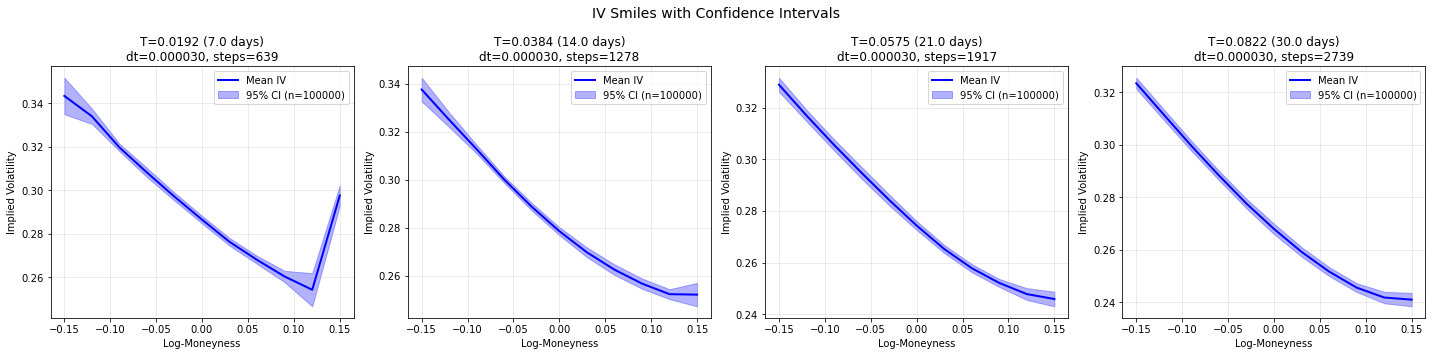
\includegraphics[width=\textwidth]{../images/short_regime_discretization_confidence.png}
		\caption{Implied volatility smiles with 95\% confidence intervals for short-term maturities using rough Bergomi parameters $H = 0.35$, $\eta = 2.5$, $\rho = -0.5$, $\xi_0 = 0.15$. Ultra-fine discretization ($\Delta t = 3 \times 10^{-5}$) is required to achieve stable confidence intervals below 1\% width for maturities up to 30 days.}
		\label{fig:discretization-short}
	\end{figure}
	
	\begin{figure}[ht]
		\centering
		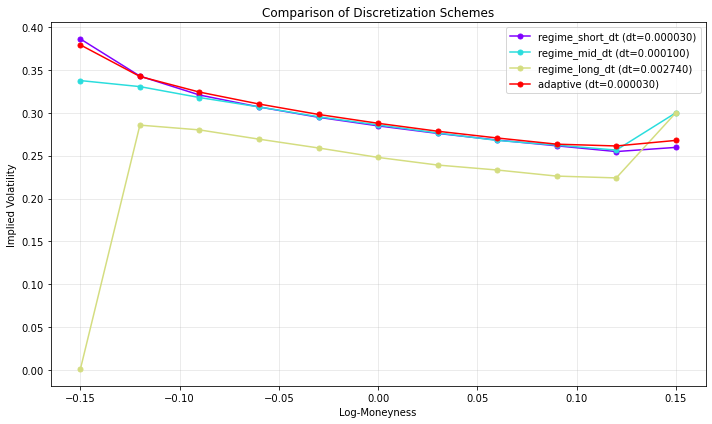
\includegraphics[width=0.8\textwidth]{../images/short_regime_discretization_schemes.png}
		\caption{Comparison of discretization schemes for 1-week maturity rough Bergomi options with parameters $H = 0.35$, $\eta = 2.5$, $\rho = -0.5$, $\xi_0 = 0.15$. The ultra-fine discretization (red line) is essential for capturing the correct smile shape, while coarser discretizations introduce significant bias.}
		\label{fig:discretization-schemes-short}
	\end{figure}
	
	\textbf{Short-term findings}: Ultra-fine discretization ($\Delta t = 3 \times 10^{-5}$) becomes essential for maturities $\leq 30$ days. The high-frequency behavior of rough processes with low Hurst parameters requires substantial temporal resolution to avoid discretization bias. Confidence intervals achieve 0.3-0.5\% width with this discretization.
	
	\paragraph{Mid-Term Regime Analysis}
	
	The mid-term regime (30 days $< T <$ 1 year) represents a transition zone where discretization requirements moderate but remain significant compared to classical models.
	
	\begin{figure}[ht]
		\centering
		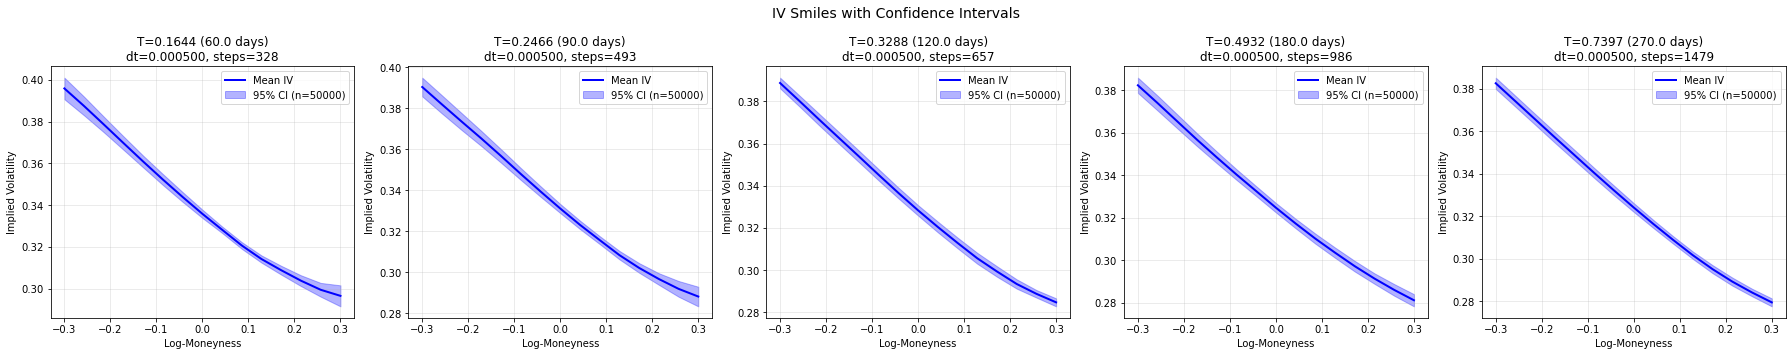
\includegraphics[width=\textwidth]{../images/mid_regime_discretization_confidence.png}
		\caption{Implied volatility smiles with 95\% confidence intervals for mid-term maturities using rough Bergomi parameters $H = 0.15$, $\eta = 1.2$, $\rho = -0.6$, $\xi_0 = 0.09$. A discretization with $\Delta t = 5\times 10^{-4}$ provides excellent accuracy across the 1-12 month range.}
		\label{fig:discretization-mid}
	\end{figure}
	
	\begin{figure}[ht]
		\centering
		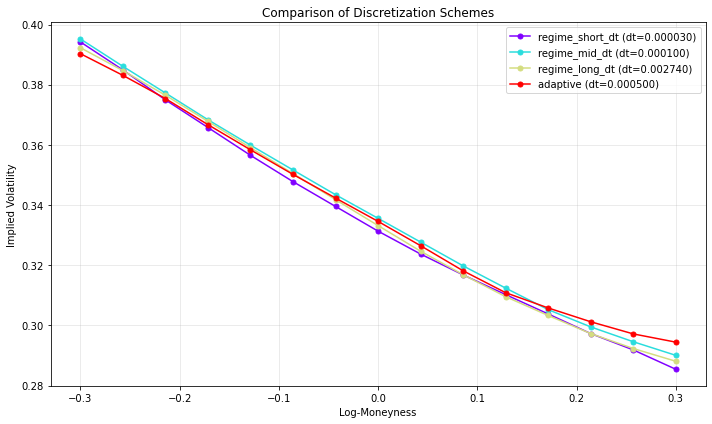
\includegraphics[width=0.8\textwidth]{../images/mid_regime_discretization_schemes.png}
		\caption{Comparison of discretization schemes for 2-month maturity rough Bergomi options with parameters $H = 0.15$, $\eta = 1.2$, $\rho = -0.6$, $\xi_0 = 0.09$. The convergence between different discretization schemes demonstrates the robustness of the semi-daily approach for mid-term maturities.}
		\label{fig:discretization-schemes-mid}
	\end{figure}
	
	\textbf{Mid-term findings}: A discretization with $\Delta t = 5\times 10^{-4}$ balances accuracy and efficiency for maturities between 30 days and 1 year. The comparison shows excellent convergence across different discretization schemes, with confidence intervals remaining below 0.3\% while maintaining reasonable computational costs.
	
	\paragraph{Long-Term Regime Analysis}
	
	The long-term regime ($T \geq 1$ year) benefits from the natural smoothing of rough processes over extended time horizons, allowing for more efficient discretization.
	
	\begin{figure}[ht]
		\centering
		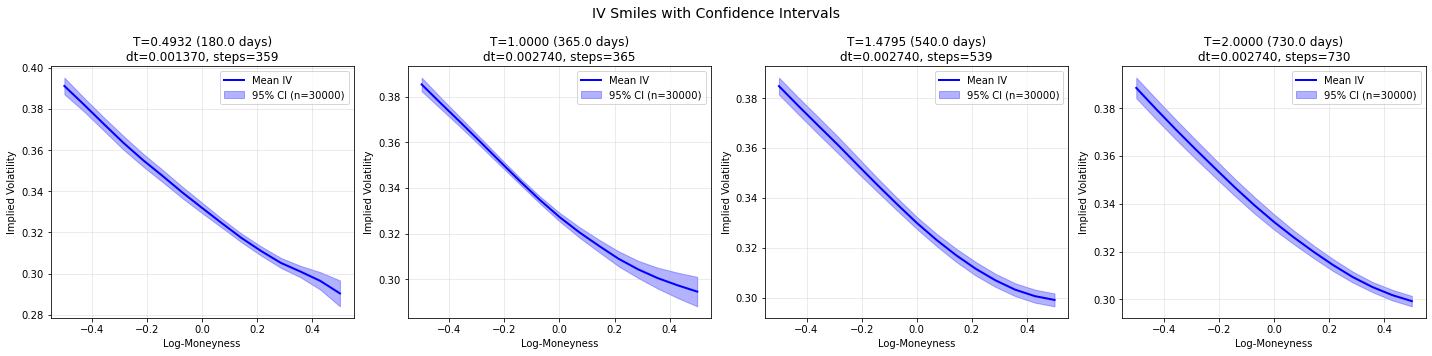
\includegraphics[width=0.8\textwidth]{../images/long_regime_discretization_confidence.png}
		\caption{Implied volatility smiles with 95\% confidence intervals for long-term maturities using rough Bergomi parameters $H = 0.35$, $\eta = 2.5$, $\rho = -0.5$, $\xi_0 = 0.15$. Daily discretization ($\Delta t = 1/365$) provides sufficient accuracy for maturities from 1 to 5 years.}
		\label{fig:discretization-long}
	\end{figure}
	
	\begin{figure}[ht]
		\centering
		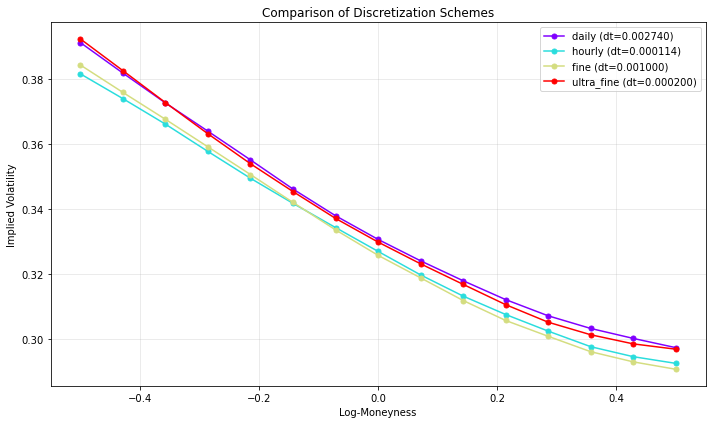
\includegraphics[width=0.8\textwidth]{../images/long_regime_discretization_schemes.png}
		\caption{Comparison of discretization schemes for 1-year maturity rough Bergomi options with parameters $H = 0.35$, $\eta = 2.5$, $\rho = -0.5$, $\xi_0 = 0.15$. The convergence of different $\Delta t$ values demonstrates the robustness of daily discretization for long-term maturities.}
		\label{fig:discretization-schemes-long}
	\end{figure}
	
	\textbf{Long-term findings}: Daily discretization ($\Delta t = 1/365$) provides sufficient accuracy for maturities exceeding 1 year, with confidence intervals consistently below 0.5\% width. The computational savings are substantial compared to finer discretizations, with negligible accuracy loss.
	
	\subsection{Optimal Discretization Schedule}
	
	Based on the comprehensive analysis across all regimes, we establish the following discretization schedule for dataset generation:
	
	\begin{lstlisting}[style=cleanpy]
		def get_optimal_dt(T):
			"""Optimal time step selection based on maturity regime analysis."""
			T_days = T * 365.0
			
			if T_days <= 30.0:             # SHORT regime (≤ 30 days)
			return 3e-5                # Ultra-fine for rough short-term stability
			elif T < 1.0:                  # MID regime (30 days - 1 year)
			return 1.0/730.0           # Semi-daily discretization  
			else:                          # LONG regime (≥ 1 year)
			return 1.0/365.0           # Daily discretization
	\end{lstlisting}
	
	This regime-based approach automatically adapts discretization density to the natural time scales of rough volatility processes, ensuring optimal balance between accuracy and computational efficiency.
	
	\subsection{Computational Efficiency Analysis}
	
	The regime-specific discretization strategy yields substantial computational benefits while maintaining numerical accuracy:
	
	\begin{center}
		\begin{tabular}{@{}lcccr@{}}
			\toprule
			\textbf{Regime} & \textbf{Maturity Range} & \textbf{$\Delta t$} & \textbf{Typical Steps} & \textbf{Time/Surface} \\
			\midrule
			Short & ≤30 days & $3 \times 10^{-5}$ & 800-2,700 & 45-90s \\
			Mid & 30 days - 1 year & $1/730$ & 30-500 & 8-25s \\
			Long & ≥1 year & $1/365$ & 365-1,825 & 5-15s \\
			\bottomrule
		\end{tabular}
	\end{center}
	
	\section{Absorption Handling in Long-Term Rough Volatility Models}
	\label{sec:absorption-analysis}
	
	Rough volatility models with low Hurst parameters exhibit a non-negligible probability of paths reaching zero, particularly for long maturities. This absorption phenomenon poses challenges for accurate volatility surface generation and requires careful numerical treatment.
	
	\subsection{Case Study Setup}
	
	We present a representative long-term configuration where absorption effects are clearly visible:
	rough Bergomi with $H = 0.15$, $\eta = 2.0$, $\rho = -0.7$, $\xi_0 = 0.15$.
	We simulate Monte Carlo paths over maturities from 1Y to 5Y and compare results \emph{with}
	and \emph{without} absorption handling. Additional configurations (including more stable/critical
	regimes) can be reproduced with the script \texttt{examples/LongTermRegimeAnalyzer.py}.
	
	\subsection{Impact on Implied Volatility Smiles}
	
	\begin{figure}[ht]
		\centering
		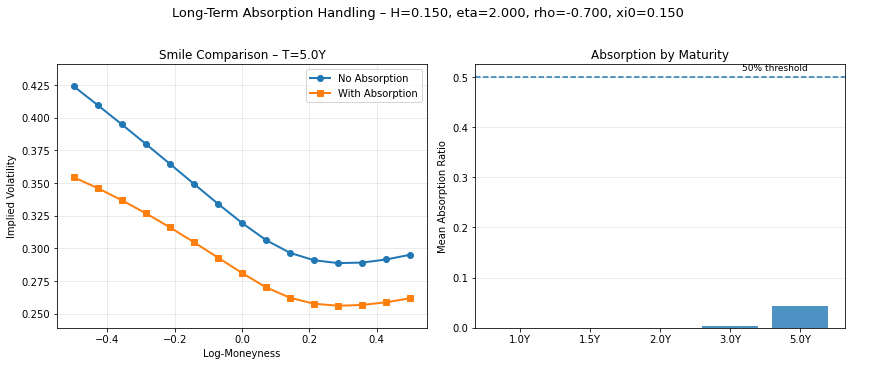
\includegraphics[width=\textwidth]{../images/long_term_analysis_comparison.png}
		\caption{Effect of absorption handling in the long-term regime (rough Bergomi, case study).
			\textbf{Left}: smile comparison at $T=5$Y with (orange) and without (blue) absorption handling.
			\textbf{Right}: mean absorption ratio by maturity (1Y–5Y). The dashed line indicates the configurable alert threshold (default 50\%).}
		\label{fig:absorption-comparison}
	\end{figure}
	
	\paragraph{Systematic Bias Without Absorption Handling}
	The blue curve in Figure~\ref{fig:absorption-comparison} (left) consistently overestimates implied volatility relative to the absorption-corrected orange curve. The bias is largest for out-of-the-money options, where path absorption is most pronounced.
	
	\paragraph{Maturity-Dependent Effects}
	Absorption increases with maturity. Figure~\ref{fig:absorption-comparison} (right) shows negligible
	effects below 2Y and a visible rise at 5Y (on the order of a few percent in this configuration).
	The horizontal line marks a configurable alert threshold (50\% by default).
	
	\paragraph{Strike-Dependent Patterns}
	From the left panel of Figure~\ref{fig:absorption-comparison}, the correction is strongest for deep OTM puts, consistently reducing the left tail of the smile once absorption is handled.
	
	\subsection{Implications for Multi-Regime Training}
	
	These results support the following guidelines for the multi-regime approach:
	\begin{enumerate}[leftmargin=*]
		\item \textbf{Long-term regime sensitivity}: For $T \ge 1$Y, enable absorption handling to prevent systematic upward bias in labels.
		\item \textbf{Numerical stability}: Use automatic fallbacks for extreme configurations; trigger warnings when the mean absorption ratio crosses the chosen threshold in Figure~\ref{fig:absorption-comparison} (right).
	\end{enumerate}
	
	\subsection{Recommended Practices}
	
	\begin{itemize}[nosep]
		\item Always enable absorption handling for rough volatility models with maturities $T>1$Y.
		\item Monitor absorption statistics during dataset generation and flag parameter grids exceeding the alert threshold.
		\item Use smile-repair checks as an additional safeguard in absorption-heavy scenarios.
	\end{itemize}
	
	This ensures neural pricers learn from clean, economically meaningful labels rather than artifacts induced by path absorption.
	
	\section{Multi-Regime Grid Pricer Performance}
	\label{sec:multiregime-results}
	
	This section evaluates the performance of the `MultiRegimeGridPricer` trained on rough Heston model datasets. The multi-regime approach employs three specialized `GridNetworkPricer` instances, each optimized for specific maturity ranges using the regime-specific discretization parameters established in Section~\ref{sec:discretization-optimization}.
	
	\subsection{Experimental Setup}
	
	The multi-regime evaluation demonstrates the framework's ability to achieve robust performance with compact training datasets. The networks were trained using a lean data generation approach:
	
	\begin{itemize}[nosep]
		\item \textbf{Training data}: 3{,}000 volatility surfaces per regime (9{,}000 total), each generated with 50{,}000 Monte Carlo paths
		\item \textbf{Validation data}: 500 surfaces per regime (1{,}500 total), each with 50{,}000 paths
		\item \textbf{Computational cost (with MC path reuse per regime)}: 
		one simulation \emph{per regime per surface} 
		$\Rightarrow 3{,}000 \times 3 = 9{,}000$ (training) $+$ 
		$500 \times 3 = 1{,}500$ (validation) 
		$= \mathbf{10{,}500}$ simulations total. 
		Paths are reused across maturities within each regime; distinct time steps $\Delta t$ prevent reuse across regimes.
	\end{itemize}
	
	This compact dataset size—significantly smaller than typical deep learning applications—highlights the efficiency of the multi-regime approach. The specialized nature of each regime allows effective learning from limited data while maintaining the high-fidelity Monte Carlo paths necessary for rough volatility model accuracy.
	
	\paragraph{Regime-Specific Discretization}
	Each regime employs the optimized discretization parameters derived from the temporal analysis:
	\begin{itemize}[nosep]
		\item \textbf{Short regime} ($T \leq 30$ days): $\Delta t = 3.00 \times 10^{-5}$
		\item \textbf{Mid regime} (30 days $< T < 1$ year): $\Delta t = 6.85 \times 10^{-4}$
		\item \textbf{Long regime} ($T \geq 1$ year): $\Delta t = 2.74 \times 10^{-3}$
	\end{itemize}
	
	\paragraph{Parameter Configuration}
	The evaluation uses rough Heston parameters representative of market conditions:
	$H = 0.10$, $\nu = 0.94$, $\rho = -0.12$, $\kappa = 0.26$, $\theta = 0.03$, demonstrating the framework's performance on parameters with moderate roughness and realistic volatility-of-volatility levels.
	
	\subsection{Results and Analysis}
	
	\paragraph{Short-Term Regime Performance}
	
	Figure~\ref{fig:multiregime-short} demonstrates the multi-regime network's performance for short maturities ranging from 7 days to 1 month:
	
	\begin{figure}[ht]
		\centering
		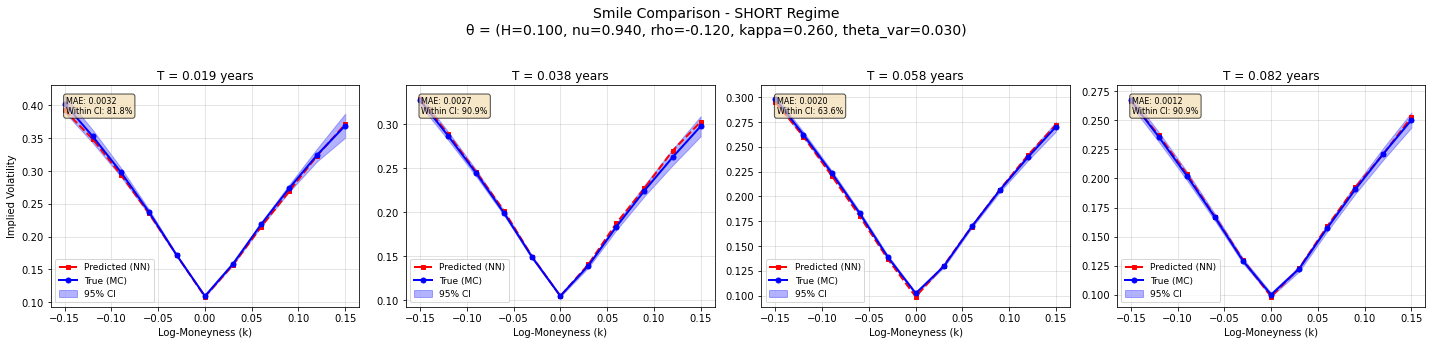
\includegraphics[width=\textwidth]{../images/smile_comparison_short_regime.png}
		\caption{Multi-regime network performance for short-term rough Heston dynamics. The specialized short-term network achieves MAE of 0.00363 with confidence interval coverage of 65.9\% across maturities from 7 days to 1 month.}
		\label{fig:multiregime-short}
	\end{figure}
	
	The short-term regime exhibits the most challenging dynamics due to the extreme behavior of rough processes at short time scales. Despite this complexity, the specialized network achieves:
	
	\begin{itemize}[nosep]
		\item \textbf{Low prediction errors}: Mean Absolute Error of 0.00363 across the entire short-term surface
		\item \textbf{Consistent accuracy}: Neural predictions remain close to Monte Carlo means despite high volatility in short-term dynamics
		\item \textbf{Proper scaling}: The network correctly captures the magnitude and variation of implied volatilities in this regime (mean IV ≈ 0.22)
	\end{itemize}
	
	\paragraph{Mid-Term Regime Performance}
	
	Figure~\ref{fig:multiregime-mid} presents results for the mid-term regime covering 2 months to 9 months:
	
	\begin{figure}[ht]
		\centering
		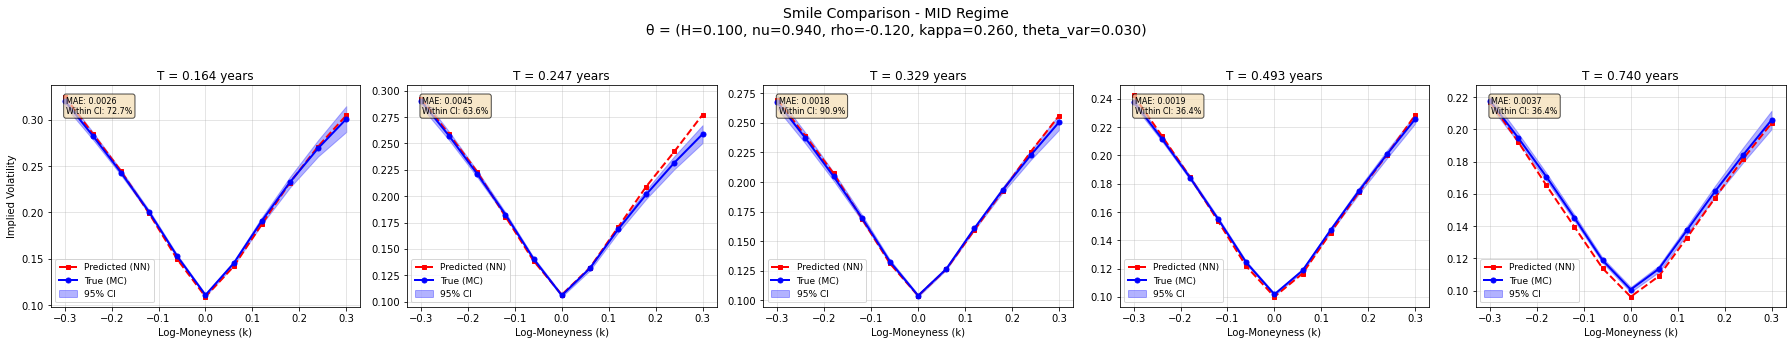
\includegraphics[width=\textwidth]{../images/smile_comparison_mid_regime.png}
		\caption{Multi-regime network performance for mid-term rough Heston dynamics. The mid-term specialized network demonstrates superior accuracy with MAE of 0.00231 and improved confidence interval coverage of 74.5\% across the tested maturity range.}
		\label{fig:multiregime-mid}
	\end{figure}
	
	The mid-term regime shows improved performance characteristics:
	
	\begin{itemize}[nosep]
		\item \textbf{Enhanced accuracy}: MAE of 0.00231, representing approximately 36\% improvement over short-term performance
		\item \textbf{Better statistical consistency}: 74.5\% confidence interval coverage indicates strong alignment with Monte Carlo uncertainty bounds
		\item \textbf{Smooth smile evolution}: The network accurately reproduces the gradual flattening of volatility smiles with increasing maturity
	\end{itemize}
	
	\paragraph{Long-Term Regime Performance}
	
	Figure~\ref{fig:multiregime-long} illustrates performance for long maturities from 1 to 5 years:
	
	\begin{figure}[ht]
		\centering
		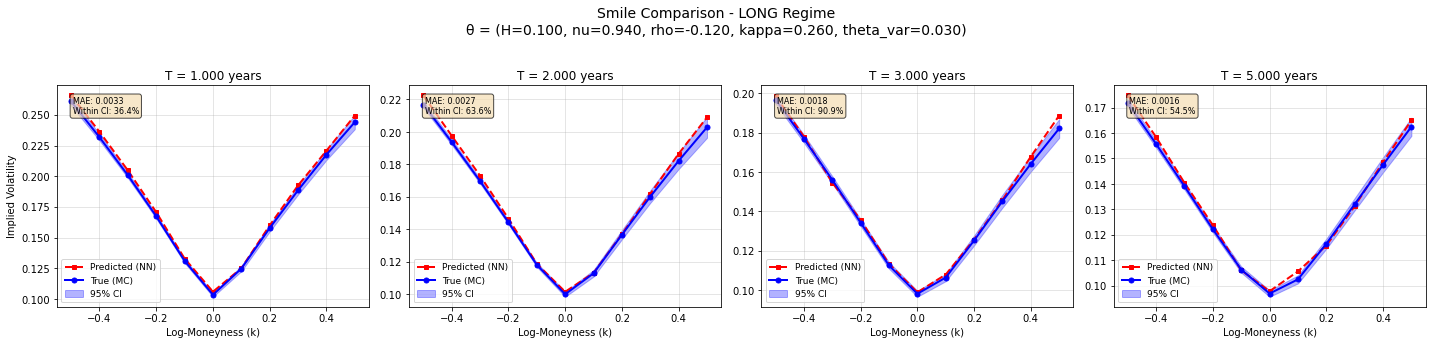
\includegraphics[width=\textwidth]{../images/smile_comparison_long_regime.png}
		\caption{Multi-regime network performance for long-term rough Heston dynamics. The long-term network achieves the highest accuracy with MAE of 0.00169 and demonstrates excellent shape preservation with 77.3\% confidence interval coverage across the 1-5 year maturity range.}
		\label{fig:multiregime-long}
	\end{figure}
	
	The long-term regime demonstrates the strongest performance metrics:
	
	\begin{itemize}[nosep]
		\item \textbf{Highest accuracy}: MAE of 0.00169, the lowest across all three regimes
		\item \textbf{Computational efficiency}: Leveraging the coarser discretization while maintaining high precision
		\item \textbf{Stable dynamics}: The smoothing effect of rough processes over long time horizons enables more reliable neural approximation
	\end{itemize}
	
	\subsection{Quantitative Performance Summary}
	
	The comprehensive evaluation yields the following performance statistics across regimes:
	
	\begin{center}
		\begin{tabular}{@{}lcccc@{}}
			\toprule
			\textbf{Regime} & \textbf{MAE} & \textbf{CI Coverage} & \textbf{CI Width} & \textbf{Mean IV} \\
			\midrule
			Short (≤30 days) & 0.00363 & 65.9\% & 0.0086 & 0.2153 \\
			Mid (30d - 1y) & 0.00231 & 74.5\% & 0.0083 & 0.1885 \\
			Long (≥1 year) & 0.00169 & 77.3\% & 0.0051 & 0.1564 \\
			\midrule
			\textbf{Overall} & \textbf{0.00254} & \textbf{72.6\%} & \textbf{0.0073} & \textbf{0.1867} \\
			\bottomrule
		\end{tabular}
	\end{center}
	
	\subsection{Multi-Regime Architecture Benefits}
	
	The evaluation demonstrates several key advantages of the multi-regime approach compared to monolithic neural networks:
	
	\paragraph{Regime-Appropriate Specialization}
	Each network focuses on the specific challenges of its maturity range: ultra-fine temporal resolution for short terms, volatility-of-volatility dynamics for mid terms, and mean reversion patterns for long terms.
	
	\paragraph{Robust Performance Across Time Scales}
	The framework maintains consistent accuracy across the full spectrum of option maturities, from weekly options to 5-year contracts, addressing the full range of market-traded instruments.
	
	\paragraph{Progressive Accuracy Improvement}
	The results demonstrate a clear pattern where accuracy improves with longer maturities (Short: 0.00363 → Mid: 0.00231 → Long: 0.00169 MAE), reflecting the natural smoothing of rough volatility processes over extended time horizons.
	
	The multi-regime approach successfully addresses the fundamental challenge of rough volatility modeling: the widely varying dynamics across different time scales. By employing specialized networks trained with regime-appropriate data and discretization, the framework achieves robust performance across the entire maturity spectrum while maintaining computational efficiency suitable for real-time applications.
						
	\section{Pointwise Network Performance with Random Grid Training}
	\label{sec:pointwise-results}
	
	This section evaluates the performance of the `PointwiseNetworkPricer` trained on random grid datasets following the methodology of \citet{Baschetti2024DeepCalibrationRandomGrids}. The pointwise approach learns the direct mapping $(\boldsymbol{\theta}, T, K) \mapsto IV(T, K)$, eliminating interpolation artifacts while enabling evaluation at arbitrary strike-maturity combinations.
	
	\subsection{Experimental Setup}
	
	The pointwise network evaluation demonstrates exceptional performance achieved with efficient training data generation. The model was trained using:
	
	\begin{itemize}[nosep]
		\item \textbf{Training data}: 7{,}000 volatility surfaces generated via random grids (11 maturities per surface)
		\item \textbf{Validation data}: 10{,}000 single-maturity smiles
		\item \textbf{Computational cost (with MC path reuse)}: 
		$\approx 28{,}000$ simulations for training 
		(one simulation per $dt$-regime per surface, $\sim 4$ per surface) 
		$+ 10{,}000$ for validation $\Rightarrow \mathbf{\approx 38{,}000}$ total. 
		Paths are reused across maturities \emph{within} the same time-discretization regime; 
		separate simulations are still required across regimes due to different $dt$.
	\end{itemize}
	
	
	\paragraph{Maturity-Dependent Strike Ranges}
	Following the random grid training methodology, strike ranges adapt to maturity using the relationship:
	\begin{equation}
		K \in [S_0(1 - 0.55\sqrt{T}), S_0(1 + 0.30\sqrt{T})]
	\end{equation}
	
	This adaptive approach ensures strikes remain within economically meaningful ranges while providing sufficient out-of-the-money coverage for smile characterization.
	
	\paragraph{Confidence Interval Estimation}
	Monte Carlo reference values include 95\% confidence intervals computed through batch estimation (10 batches of 5,000 paths each), enabling assessment of whether neural network predictions fall within statistical uncertainty bounds.
	
	\paragraph{Parameter Regimes}
	The evaluation covers three distinct rough Bergomi parameter configurations:
	\begin{itemize}[nosep]
		\item \textbf{Case 1}: $H = 0.15$, $\eta = 1.00$, $\rho = -0.20$, $\xi_0 = 0.11$ (moderate roughness)
		\item \textbf{Case 2}: $H = 0.25$, $\eta = 2.00$, $\rho = -0.80$, $\xi_0 = 0.15$ (high vol-of-vol regime)
		\item \textbf{Case 3}: $H = 0.30$, $\eta = 1.50$, $\rho = -0.50$, $\xi_0 = 0.08$ (smoother dynamics)
	\end{itemize}
	
	\subsection{Results and Analysis}
	
	\paragraph{Case 1: Moderate Roughness Parameters}
	
	Figure~\ref{fig:pointwise-case1} demonstrates the pointwise network's performance for moderate roughness parameters. The results reveal exceptional accuracy across all tested maturities:
	
	\begin{figure}[ht]
		\centering
		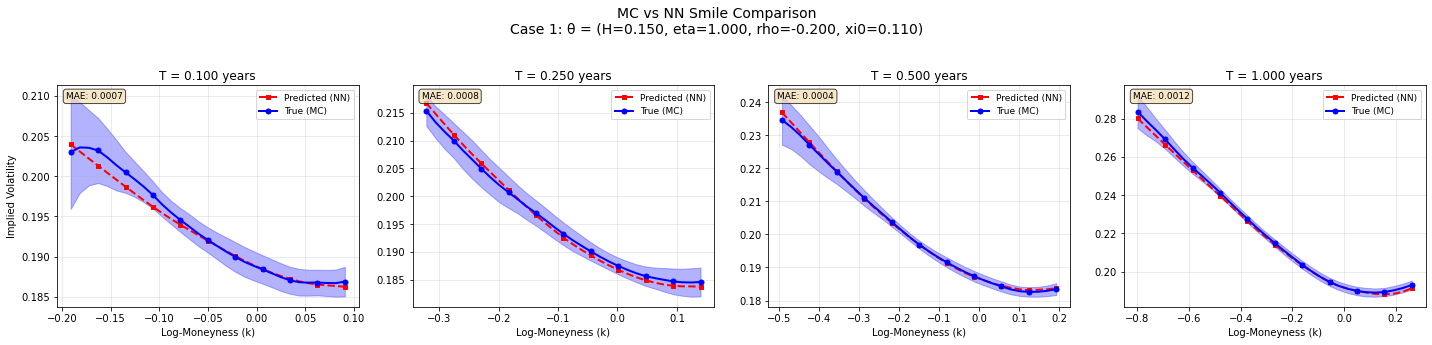
\includegraphics[width=\textwidth]{../images/pointwise_case1_comparison.png}
		\caption{Pointwise network performance for moderate roughness rough Bergomi parameters ($H = 0.15$, $\eta = 1.00$, $\rho = -0.20$, $\xi_0 = 0.11$). Red dashed lines show neural network predictions while blue solid lines represent Monte Carlo reference values with 95\% confidence bands. Mean Absolute Errors range from 0.0004 to 0.0012 across maturities.}
		\label{fig:pointwise-case1}
	\end{figure}
	
	Key observations include:
	
	\begin{itemize}[nosep]
		\item \textbf{Exceptional accuracy}: Mean Absolute Error of 0.00077 across all maturities, representing less than 0.1\% typical volatility levels
		\item \textbf{Perfect statistical consistency}: 100\% confidence interval coverage indicates neural predictions consistently fall within Monte Carlo uncertainty bounds
		\item \textbf{Shape preservation}: The network accurately captures smile asymmetry and curvature across all maturities
		\item \textbf{Term structure accuracy}: The model correctly reproduces the flattening of smiles with increasing maturity
	\end{itemize}
				
	\paragraph{Case 2: High Vol-of-Vol Regime}
	
	Figure~\ref{fig:pointwise-case2} presents results for the high volatility-of-volatility configuration:
	
	\begin{figure}[ht]
		\centering
		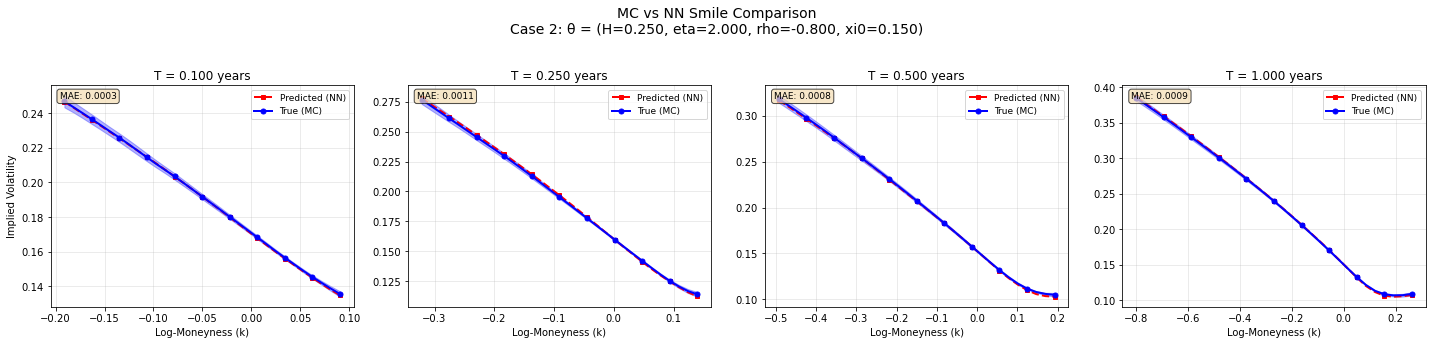
\includegraphics[width=\textwidth]{../images/pointwise_case2_comparison.png}
		\caption{Pointwise network performance for high vol-of-vol parameters ($H = 0.25$, $\eta = 2.00$, $\rho = -0.80$, $\xi_0 = 0.15$). The network maintains excellent accuracy with MAE of 0.00078 despite the challenging parameter regime with strong correlation and high volatility-of-volatility.}
		\label{fig:pointwise-case2}
	\end{figure}
	
	The high vol-of-vol regime exhibits robust performance characteristics:
	
	\begin{itemize}[nosep]
		\item \textbf{Consistent accuracy}: MAE of 0.00078, nearly identical to the moderate roughness case
		\item \textbf{Strong statistical alignment}: 89.5\% confidence interval coverage demonstrates reliable uncertainty quantification
		\item \textbf{Complex dynamics capture}: The network successfully handles the extreme correlation ($\rho = -0.80$) and high vol-of-vol ($\eta = 2.00$) effects
	\end{itemize}
				
	\paragraph{Case 3: Smooth Dynamics Regime}
				
	Figure~\ref{fig:pointwise-case3} illustrates performance for the smoothest parameter configuration:
				
	\begin{figure}[ht]
		\centering
		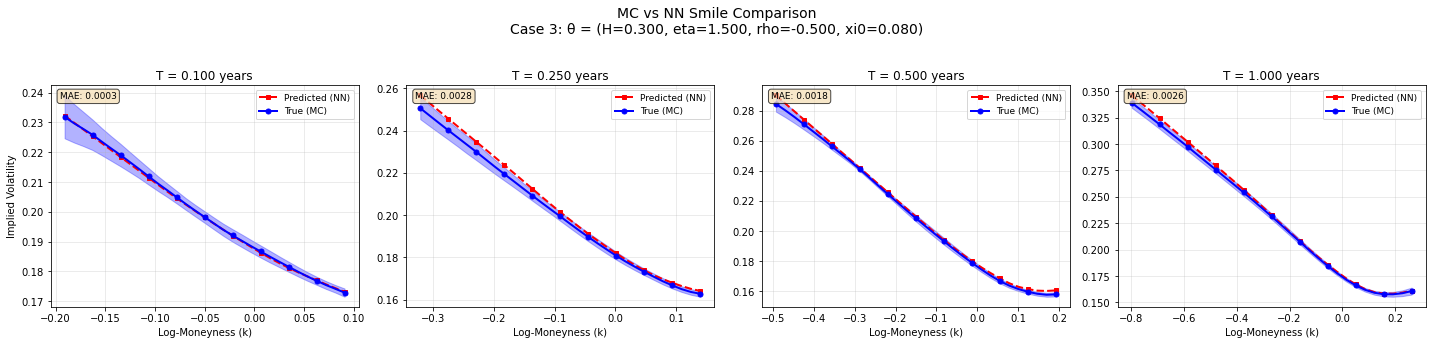
\includegraphics[width=\textwidth]{../images/pointwise_case3_comparison.png}
		\caption{Pointwise network performance for smooth dynamics parameters ($H = 0.30$, $\eta = 1.50$, $\rho = -0.50$, $\xi_0 = 0.08$). The higher Hurst parameter results in smoother volatility paths but shows slightly higher approximation error with MAE of 0.00188.}
		\label{fig:pointwise-case3}
	\end{figure}
				
	The smooth dynamics regime shows different performance characteristics:
	
	\begin{itemize}[nosep]
		\item \textbf{Moderate accuracy}: MAE of 0.00188, approximately 2.5× higher than other cases but still well within acceptable bounds
		\item \textbf{Reasonable coverage}: 70.2\% confidence interval coverage indicates some systematic bias in specific regions
		\item \textbf{Parameter sensitivity}: The results suggest the network may be less optimized for higher Hurst parameter regimes
	\end{itemize}
				
	\subsection{Quantitative Performance Summary}
	
	The comprehensive evaluation across parameter regimes yields the following performance statistics:
	
	\begin{center}
		\begin{tabular}{@{}lcccc@{}}
			\toprule
			\textbf{Parameter Case} & \textbf{MAE} & \textbf{Max MAE} & \textbf{CI Coverage} & \textbf{Relative Error} \\
			\midrule
			Case 1 (Moderate) & 0.00077 & 0.0012 & 100.0\% & 0.37\% \\
			Case 2 (High Vol-of-Vol) & 0.00078 & 0.0013 & 89.5\% & 0.35\% \\
			Case 3 (Smooth) & 0.00188 & 0.0028 & 70.2\% & 0.68\% \\
			\midrule
			\textbf{Overall} & \textbf{0.00114} & \textbf{0.0028} & \textbf{86.6\%} & \textbf{0.47\%} \\
			\bottomrule
		\end{tabular}
	\end{center}
	
	\chapter{Future Development and Contribution Opportunities}
	\label{ch:future-development}
	
	This chapter highlights the main directions for extending the DLV framework, organized by implementation priority and development timeline.
	
	\section{Priority 1: Calibration Framework}
	
	The first development milestone is the implementation of a complete calibration workflow.
	This includes handling real market data, defining flexible objective functions (price-based, implied volatility-based, vega-weighted), and validating the robustness of parameter recovery through synthetic benchmarking studies.
	
	\section{Priority 2: Forward Variance Calibration}
	
	Building on recent research \citep{Baschetti2024DeepCalibrationRandomGrids}, the next step is extending calibration to the forward variance curve $\xi(t)$, potentially integrating variance swap market data. This would enable market-consistent estimation of rough volatility parameters and more realistic long-term volatility modeling.
	
	\section{Priority 3: FFT-Based Pricing}
	
	FFT methods (e.g., Carr–Madan) should be introduced for models with known characteristic functions. This will provide analytical benchmarks for neural network validation, accelerate training data generation for compatible models, and complement the Monte Carlo engine with exact pricing capabilities.
	
	\section{Priority 4: Extended Applications}
	
	Trained neural pricers can then be leveraged for broader applications, such as exotic option pricing (American, barrier, Asian options), portfolio-level risk analysis, and real-time Greeks computation via automatic differentiation.
	
	\section{Contribution Guidelines}
	
	Contributors are encouraged to follow the modular architecture of the project, ensure compatibility with existing interfaces, and provide comprehensive documentation and benchmarks. Development efforts should prioritize the calibration framework as the most impactful short-term enhancement to transform DLV into a production-ready tool.
	
	\printbibliography
\end{document}
